\documentclass[12pt]{article}
\usepackage[margin=1in]{geometry}
\usepackage{amsmath,amsthm,amssymb,amsfonts}
\usepackage{graphicx}
\usepackage{physics}
%\usepackage{halloweenmath}
\usepackage{setspace}
\usepackage[font=small,labelfont=bf]{caption}

\newcommand{\N}{\mathbb{N}}
\newcommand{\Z}{\mathbb{Z}}

\newenvironment{part}[2][Part]{\begin{trivlist}
\item[\hskip \labelsep {\bfseries #1}\hskip \labelsep {\bfseries #2.}]}{\end{trivlist}}
%If you want to title your bold things something different just make another thing exactly like this but replace "problem" with the name of the thing you want, like theorem or lemma or whatever

\graphicspath{ {../} }

\begin{document}

\title{\textbf{ASTR 522: Dark Current Lab}}
\author{Jonas Powell}
\maketitle


%\twocolumn
\begin{onehalfspacing}



%~~~~~~~~~~~~~~~~~~~~~~~~~~~~~~~~~~~~~~~~~~~~~~~~~~~~~~~~~~~~~~~~~~~~~~~~~~~~
\raggedright{\textbf{\Large Part 1:}} \\
\raggedright{\textbf{\large Measuring the Read Noise}}
Selected values for $p_{lo}, p_{hi}$: 0, 50000 \\
Image min: 1861
Image max: 4766
Image mean: 1910.79
Image std. dev: 10.73

 Selected values for $p_{lo}, p_{hi}$: 1861, 2000 \\
 Image min: 1861
 Image max: 2000
 Resulting statistics: \\
 Image mean: 1910.78
 Image std dev: 10.29

 \begin{figure}[h!]
     \centering
     \begin{minipage}{0.48\textwidth}
         \centering
         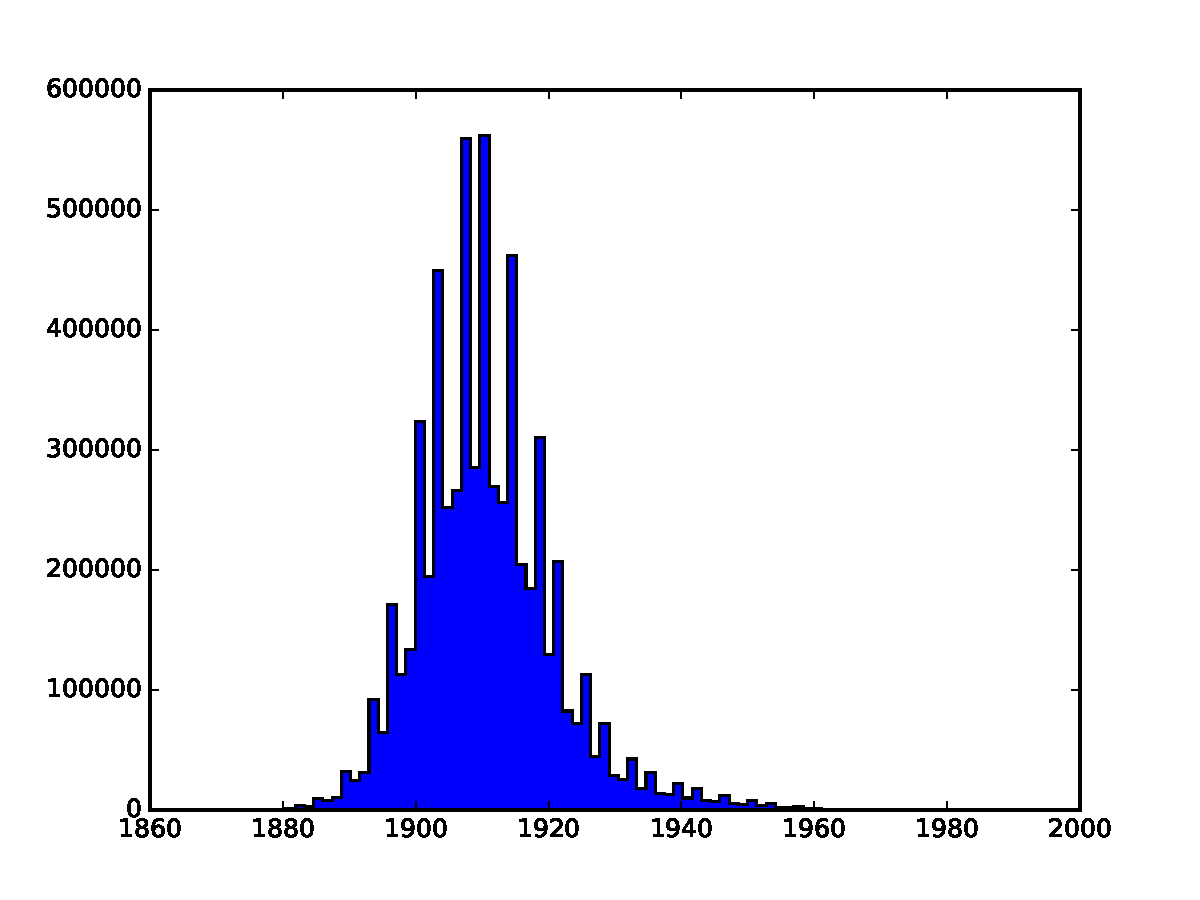
\includegraphics[width=1.05\textwidth]{part1_hist} % first figure itself
         \caption{SED for the quasar 3C273.}
     \end{minipage}\hfill
     %\iffalse
     \begin{minipage}{0.48\textwidth}
         \centering
         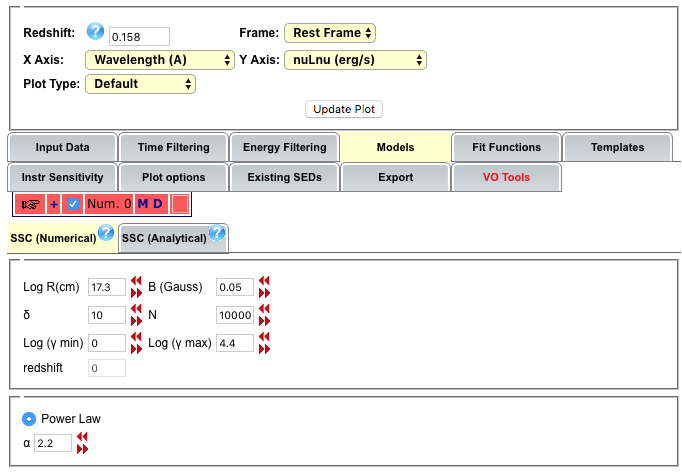
\includegraphics[width=0.75\textwidth]{part1_params} % second figure itself
         \caption{SED for the quasar 3C273 with Composite QSO template applied and ARO=0.61}
     \end{minipage}\hfill
   %\fi
 \end{figure}


Examine the image in DS9. Is the std. deviation dominated by random fluctuations or groups (i.e. bad columns)?


DIFF stuff:


 \begin{figure}[h!]
     \centering
     \begin{minipage}{0.48\textwidth}
         \centering
         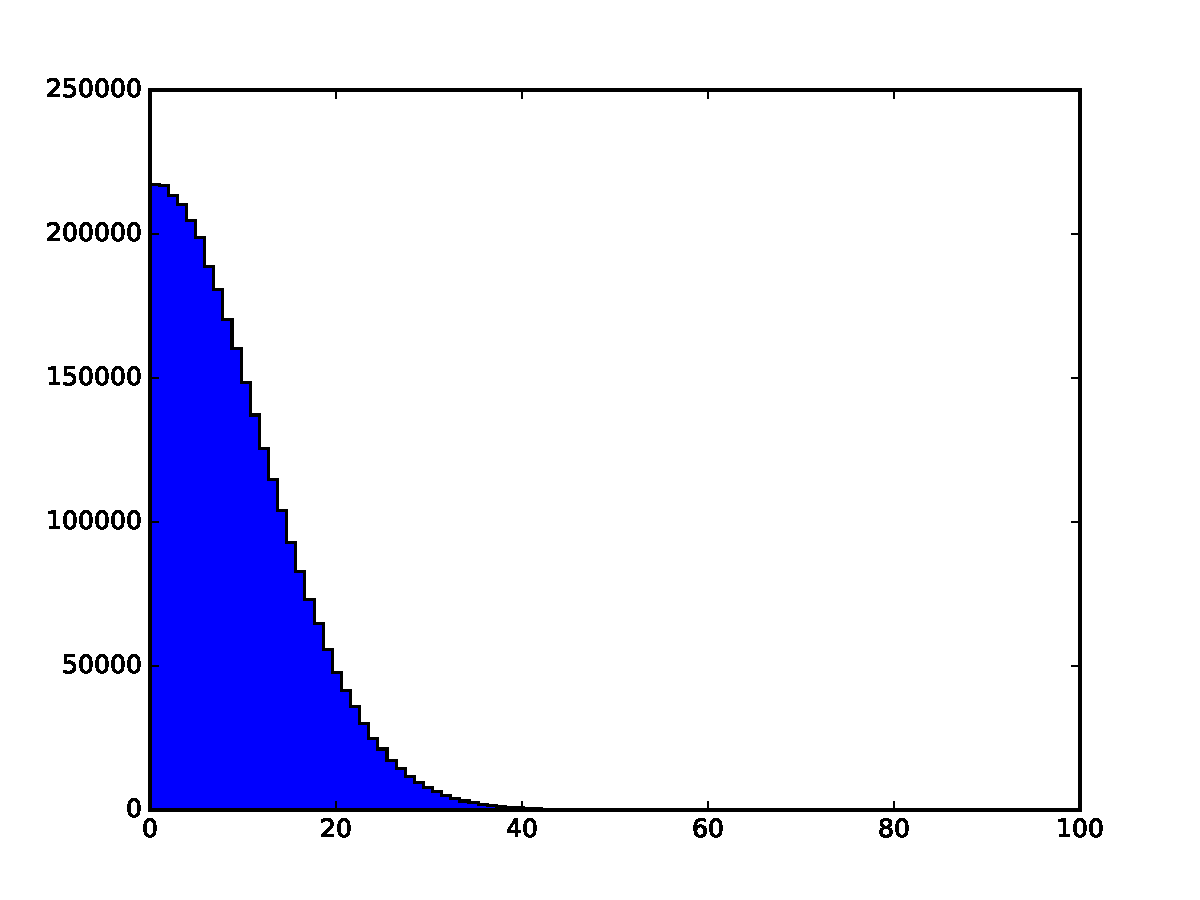
\includegraphics[width=1.05\textwidth]{part1_diff-hist} % first figure itself
         \caption{SED for the quasar 3C273.}
     \end{minipage}\hfill
     %\iffalse
     \begin{minipage}{0.48\textwidth}
         \centering
         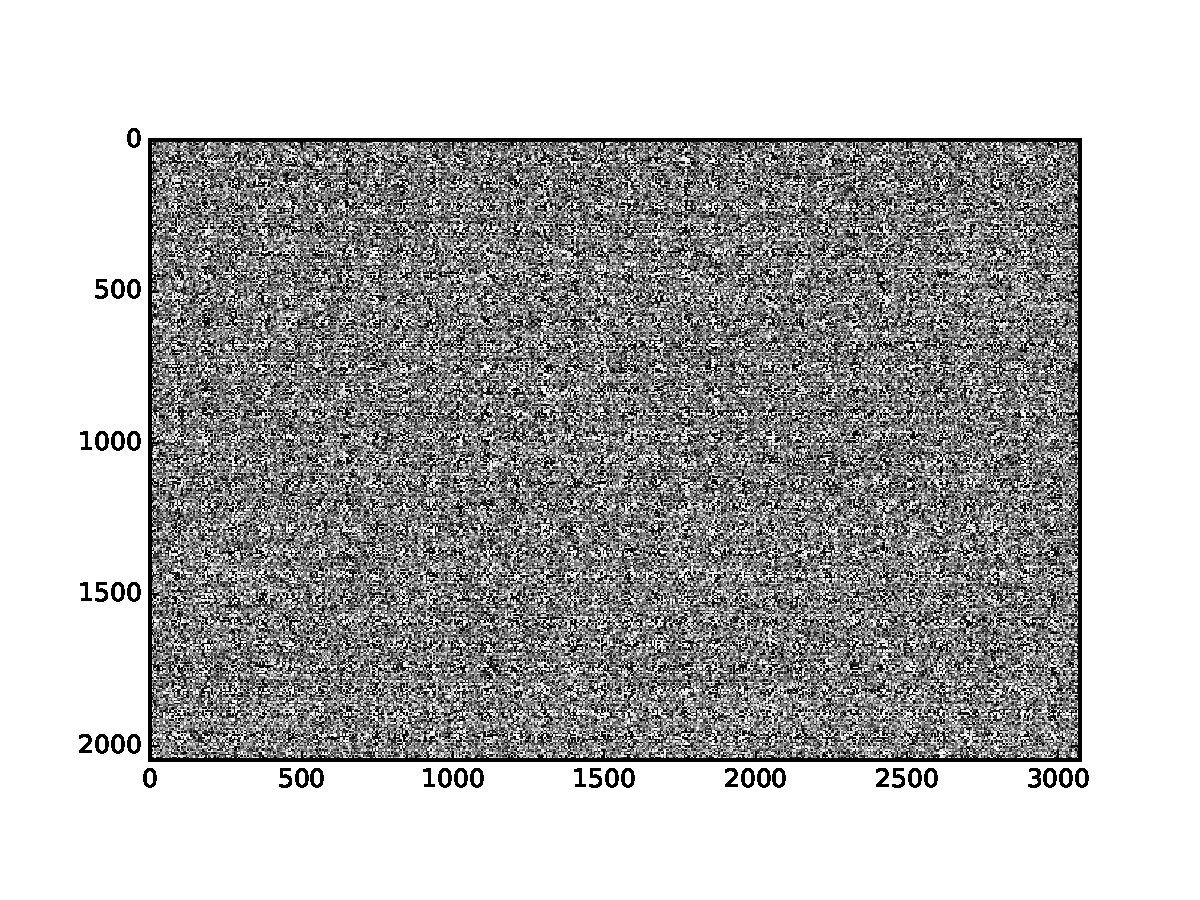
\includegraphics[width=0.75\textwidth]{part1_diff-field} % second figure itself
         \caption{SED for the quasar 3C273 with Composite QSO template applied and ARO=0.61}
     \end{minipage}\hfill
   %\fi
 \end{figure}










\end{onehalfspacing}

\end{document}
